    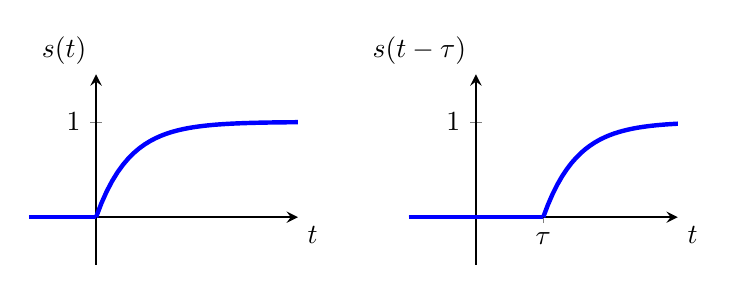
\begin{tikzpicture}
        \begin{axis}[
        name=ax2,
        axis line style = thick,
        height=4cm,
        width=5cm,
        axis x line=center,
        axis y line=center,
        xmin=-2,
        xmax=6,
        ymin=-0.5,
        ymax=1.5,
        ytick={1},
        yticklabels={$1$},
        xtick=\empty,
        xlabel={$t$},
        ylabel={$s(t)$},
        xlabel style={below right},
        ylabel style={above left},
        ]
        \addplot [ultra thick,color=blue,domain=-2:0, samples=101,unbounded coords=jump]{0};
            \addplot [ultra thick,color=blue,domain=0:16, samples=101,unbounded coords=jump]{1-exp(-x)};
%	\draw[dotted,ultra thick,blue] (axis cs:0,0) -- (axis cs:0,1);
        \end{axis}
        \begin{axis}[
        at={(ax2.south east)},
        xshift=4em,
        ytick=\empty,
        axis line style = thick,
        height=4cm,
        width=5cm,
        axis x line=center,
        axis y line=center,
        xmin=-2,
        xmax=6,
        ymin=-0.5,
        ymax=1.5,
        ytick={1},
        yticklabels={$1$},
        xlabel={$t$},
        ylabel={$s(t-\tau)$},
        xlabel style={below right},
        ylabel style={above left},
	xticklabels={$\tau$},
        xtick={2},
        ]
        \addplot [ultra thick,color=blue,domain=-2:2, samples=101,unbounded coords=jump]{0};
            \addplot [ultra thick,color=blue,domain=2:16, samples=101,unbounded coords=jump]{1-exp(-(x-2))};
%	\draw[dotted,ultra thick,blue] (axis cs:2,0) -- (axis cs:2,1);
        \end{axis}
    \end{tikzpicture}
